\begin{itemize}
    \item EDs 1er orden:
        \[
          \frac{d y}{d x} = f(x,y) = e^x\sin\p{ y } 
        \]
    
    \item Solución general: 
        \[
          \phi(x,y)+C
        \]
    \item Solución particular: son libres de constantes.
\end{itemize}
Son necesarias condiciones en la variable $y(x_0)=y_0$  y sus derivadas para no tener constantes arbitrarias.

\subsection{Problema de valor inicial (PVI) de primer orden}
\begin{itemize}
    \item Es una ED de 1er orden con una condición inicial.
        \[
          \frac{d y}{d x} = f(x,y), \qq y(x_0) = y_0
        \]
\end{itemize} 

\subsection{PVI de 2do grado}
\[
  \frac{d ^2y}{d x^2} = f(x,y,y'), \qq y(x_0)=y_0 11 y'(x_0)=V_0
\]
En física, tienen la aceleración $y''$ $y$ quieren encontrar el desplazamiento. Se necesita la posición inicial $y(0)=y_0$ y la velocidad inicial $y'(0)=V_0$.

\subsection{Ejercicio 1: Encuentre la solución particular de las sigs EDs.}
\begin{itemize}
    \item $\displaystyle y'=y-y^2$, $\displaystyle y(-1)=5$ Use la solución general: $\displaystyle y(x)=\frac{1}{1+ce^{-x}}$ 
        \begin{itemize}
            \item Recordar que lo único que tenemos que hacer es encontrar la constante de la solución general.
        \end{itemize}
        \begin{center}
           \begin{align*}
               \text{ Use: } \qq x=-1, \qq y=5 \qq \text{ para encontrar el valor de C. } \\ 
               \frac{1}{1+ce^1}=5 \qimplies 1+ce^1=\frac{1}{5} \\ 
               ce=\frac{1}{5}-1 \qimplies  c= -\frac{4}{5e} \\ 
               \text{ Solución particular: } \qq y(x)=\frac{1}{1-\frac{4}{5e}e^{-x}} \\ 
           \end{align*}
        \end{center}
    
    \item $\displaystyle u''+u=0, \qq u(\pi/2)=2, \qq u'(\pi/2)=5$ Use la solución general $\displaystyle u = c_1\sin\p{ x } +c_2\cos\p{ x } $.
        \begin{center}
           \begin{align*}
               u' = c_1\cos\p{ x } -c_2\sin\p{ x } \\ 
               \text{ Aplique cada una de las CIs. } \\ 
               u(\pi/2) = c_1\cdot 1 + c_2\cdot 0 \qimplies  c_1 = 2 \\ 
               u'(\pi/2) = c_1\cdot 0 - c_2\cdot 1 = 5 \qimplies c_2 = -5 \\ 
               \text{ Solución particular: } u(x) = 2\sin\p{ x } -5\cos\p{ x } \\ 
           \end{align*}
        \end{center}
\end{itemize}


\subsection{Resolución de una ED}
Casos:
\begin{enumerate}
    \item Solución única.
    \item Infinitas soluciones.
    \item No hay solución, ocurre en un PVI (usualmente cuando se ponen condiciones imposibles).
\end{enumerate}

\begin{itemize}
    \item No todos los problemas con valor inicial con condiciones tienen soluciones únicas.
    \item Por ejemplo: $\displaystyle \frac{d y}{d t} =3y^{2/3}$  sujera a $y(0)=0$ tiene por lo menos 2 soluciones. $y(t)=0 \qq y(t)=t^3$.
        \begin{itemize}
            \item ¿Cómo sabemos que es $t^3$?
                \begin{center}
                   \begin{align*}
                       \frac{dy}{3y^{2/3}}=dt \qq \text{ integrar. } \\ 
                        \int_{}^{}\frac{1}{3}y^{-2/3}dy = \int_{}^{}dt \\ 
                        \frac{3}{3}y^{1/3} = t + c \\ 
                        y = (t+c)^3 \qq \text{ Solución general } \\ 
                        0 = (0 + c)^3 \qimplies c^3=0 \qimplies c=0 \\ 
                        \text{ Solución particular: } \qq y = t^3 \\ 
                   \end{align*}
                \end{center}
        \end{itemize}
\end{itemize}

\subsection{¿Cuándo un PVI tiene garantizada solución única?}
\begin{itemize}
    \item El problema de valor inicial de primer orden $y'=f(x,y)$ $y(x_0)=y_0$ tiene garantizada una solución única si $f(x,y)$ y $\frac{\delta f}{\delta y} $ son continuas en $(x_0,y_0)$.
\end{itemize}

\subsection{Ejercicios}
Ejercicio 2a: Encuentre y grafique los puntos $(x,y)$ donde la solución única del PVI está garantizada.
\begin{itemize}
    \item $\displaystyle y'=y-y^2$ 
        \begin{center}
           \begin{align*}
               f(x,y)=y-y^2 \qq \text{ es continua en } \qq \mathbb{R^2} \\ 
               \frac{\delta f}{\delta y} = 1-2y \qq \text{ es continua en } \qq \mathbb{R^2} \qq \text{(plano)} \\ 
               \text{ La solución única está garantizada en: } \qq -\infty<x<\infty \qq -\infty<y<\infty \\ 
           \end{align*}
           \begin{figure}[H]
               \centering
               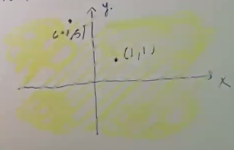
\includegraphics[width=0.4\textwidth]{./Figs/2021-01-13-10-35-55.png}
           % 	\caption{}
           \end{figure}
        \end{center}
    
    \item $\displaystyle y'=3y^{2/3}$ 
        \begin{center}
           \begin{align*}
               f(x,y)=3y^{2/3} \qq \text{ es continua en $\mathbb{R}^2$ } \\ 
               \text{ Pero: } \qq \frac{\delta f}{\delta y} = \frac{3\cdot 2}{3}y^{-1/3} = \frac{2}{y^{1/3}} \\ 
               \text{ No es continua en $y=0$. No hay solución garantizada si $y=0$ $(x,y), y\neq 0$. } \\ 
           \end{align*}
        \end{center}
    
    \item $\displaystyle y'=\frac{\sqrt{y^4-16}}{x}$ 
        \begin{itemize}
            \item Evite números negativos.
            \item Evite denominador igual a cero.
        \end{itemize}
        \begin{center}
           \begin{align*}
               f(x,y) = \frac{\sqrt{y^4-16}}{x} \qq \text{ no es continua en x=0 \& -2<y<2 } \\ 
               y^4-16 \geq 0 \qimplies y^4 \geq 16 \qimplies -2\geq y \geq 2 \\ 
               \text{ Adicionalmente: } \frac{\delta f}{\delta y} = \frac{1}{x}(y^4-16)^{-1/2} \frac{1}{2}4y^3 \\ 
               \frac{\partial f}{\partial y} = \frac{2y^3}{x\sqrt{y^4-16}} \qq \text{ se indefine en: }\qq \pm 2 \\ 
               \text{ Solución garantizada si } \qq x=0 \qq -2\leq y \leq2 \\ 
           \end{align*}
           \begin{figure}[H]
               \centering
               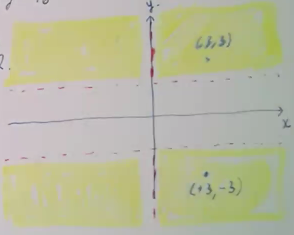
\includegraphics[width=0.4\textwidth]{./Figs/2021-01-13-10-47-35.png}
           % 	\caption{}
           \end{figure}
        \end{center}
\end{itemize}

\subsection{ED separable de primer orden}
\[
  \frac{d y}{d x} = f(x)g(y)
\]
\begin{itemize}
    \item el lado derecho es un producto de dos funciones en $x$ y en $y$.
    \item ED lineal de 1er orden.
        \[
          a(x)\frac{d y}{d x} + b(x)y = c(x)
        \]
    
    \item Las funciones coeficientes $a,b,c$ sólo dependen de x.
        \[
          \frac{d y}{d x} \qq \text{ \& } \qq y \qq \text{ sólo tienen potencias de uno. }
        \]
    
    \item ED exacta:
        \[
          M dy + N dx = 0  \qq \frac{\partial M}{\partial x} = \frac{\partial N}{\partial y} \\ 
        \]
    
    \item Una ED de 1er orden $\displaystyle \frac{d y}{d x} = f(x,y)$ se puede escribir usando diferenciales. La idea es tratar el $dy,dx$ como una fracción.
        \[
          dy=f(x,y)dx \qimplies dy=f(x,y)dx=0
        \]
\end{itemize}

\subsection{Ejercicio 3}
Determine si la ED dada es lineal o es separable.
\begin{enumerate}
    \item $\displaystyle (y-x^2)dx+4ydy = 0$
        \begin{center}
           \begin{align*}
               (y-x^2)dx+4xdy = 0 \\ 
               (y-x^2)+4x\frac{d y}{d x} =0 \\ 
               4x\frac{d y}{d x} = x^2-y \\ 
               \frac{d y}{d x} = \frac{x^2-y}{4x} \qimplies \text{ No es separable por el término $x^2-y$} \\ 
           \end{align*}
           \begin{itemize}
               \item Pero sí es lineal.
           \end{itemize}
           \begin{align*}
                4x\frac{d y}{d x}  + y = x^2 \\ 
                a(x) = 4x, \qq b(x) = 1, c(x) = x^2 \\ 
           \end{align*}
        \end{center}
    
    \item $\displaystyle ydx+(x+xy+e^y)dy=0$ 
        \begin{center}
           \begin{align*}
               y + \underbrace{(x+xy+e^y)}_{a(x)}\frac{d y}{d x} = 0 \qq \text{ No es lineal. } \\ 
               (x+xy+e^y)\frac{d y}{d x} = -y
               \frac{d y}{d x} = \frac{-y}{(x+xy+e^y)} \qq \text{ No es separable. } \\ 
           \end{align*}
        \end{center}
    
    \item $\displaystyle ydx+(xxye^y)dy=0$ 
        \begin{center}
           \begin{align*}
               x^2ye^y\frac{d y}{d x} +y = 0 \qq \text{ No es lineal. } \\ 
               \frac{d y}{d x} = \frac{-y}{x^2ye^y} = -\frac{1}{x^2e^y} = \p{-\frac{1}{x^2}} \p{\frac{1}{e^y}} \qq \text{ Es separable. } \\ 
               \text{ Separe en términos de $x$ \& de $y$. } \\ 
               e^ydy=-\frac{1}{x^2}dx \\ 
               \int e^ydy=\int -x^{-2}dx \\ 
               e^y + c_1 = x^{-1} + c_2 \\ 
               y = \ln\p{ c_2 - c_1 + \frac{1}{x} } \qimplies \text{ Solución general. } \\ 
           \end{align*}
        \end{center}
\end{enumerate}
